\documentclass{article}
\usepackage{graphicx}
\usepackage{amsmath}

\title{Simulation and Analysis of Energy Deposition in a Particle Detector}
\author{Derek Grove}
\date{\today}

\begin{document}

\maketitle

\section*{Introduction}

In the field of high-energy physics, understanding the response of particle detectors to a high energy particle beam is critical. When charged particles pass through the detector, they deposit energy, which is then measured to provide information about the incoming particles. This paper presents a simulation of energy deposition in a particle detector, focusing on the distribution of deposited energy and the uncertainties associated with its measurement.

\section*{Experiment Simulation}

The simulation is based on the premise that the true energy deposition follows a Landau distribution, which is typical for ionizing radiation passing through matter. We represent this distribution with a mean of 50 GeV and a standard deviation of 3 GeV. These are arbitrarily chosen, thin detectors (like silicon detectors) have very little energy deposited in them whereas calorimeters absorb far more. For simplicity, I'm just making a toy detector that on average absorbs 50 GeV. 

In addition to the randomly distributed energy deposition, the measurement of energy deposition is not perfect and is subject to uncertainties. In our simulation, we model this uncertainty using a Poisson distribution. The Poisson distribution is appropriate because the energy deposition is a counting process, where the number of energy quanta deposited in the detector can be considered as independent random events. In addition to statistical fluctuations like our Poisson fluctuations, there are many other sources of uncertainty we considered but decided not to model. To name a few: 

\begin{enumerate}
    \item \textbf{Systematic Uncertainties:} These can arise from various sources such as inaccuracies in the detector calibration, non-uniformities in detector response, uncertainties in the beam energy, etc.
    \item \textbf{Measurement Noise:} The detectors and the electronics associated with them will have inherent noise which will contribute to the uncertainty. This is particularly relevant when the signal is small compared to the noise level.
    \item \textbf{Modeling Uncertainties:} These arise from the assumptions and approximations made in modeling the physics processes involved in the experiment. For instance, the uncertainty in the cross-sections used in the Monte Carlo simulations, uncertainties in the physics models used to describe particle interactions in the detector, etc.
    \item \textbf{Data Analysis Uncertainties:} These come from the methods used to extract the quantities of interest from the raw data. For example, if you are fitting a function to your data to extract parameters, the uncertainties in the fit parameters contribute to the overall uncertainty.
    \item \textbf{Beam Position and Profile Uncertainty:} The exact position and profile (spread) of the beam can also contribute to uncertainties, particularly if the beam isn't perfectly uniform or if there's any drift in the beam position over time.
\end{enumerate}


In our simplified model with only Poisson fluctuations, we scaled down said fluctuations to model smaller uncertainties. This is an assumption on our part, its just that the default smearing function in ROOT made very large error bars, maybe these are realistic, but we decided to scale them down. The scale factor of 0.2 is chosen arbitrarily, but it could be adjusted based on more detailed knowledge about the detector's response.

For the sake of physics, we pretend we do not know that our distribution is Landau, we would like to pretend as though this is raw data from a real detector and we must now model it with our computational skills.

\section*{Analysis of Simulation Results}

After generating the smeared energy deposition data, we fit it using three different functions: a Gaussian, a Landau, and a Crystal Ball function. The Gaussian function represents the simplest assumption about the distribution, while the Landau function represents something a little more specific (long tail into the higher energies). The Crystal Ball function, which is a combination of a Gaussian core with a power-law tail, is often used to model detector responses that may have long tails due to rare, large energy deposition events, or even momentum distributions.

For each fit, we calculate the reduced chi-square value to quantify the goodness of fit. The Gaussian fit yielded a reduced chi-square value of 1820.84, indicating a poor fit to the data. The Landau fit, on the other hand, had a reduced chi-square value of 1.55, and the Crystal Ball fit had a value of 1.76. These latter two values suggest a good fit to the data, as they are close to 1.

\begin{figure}[h!]
    \centering
    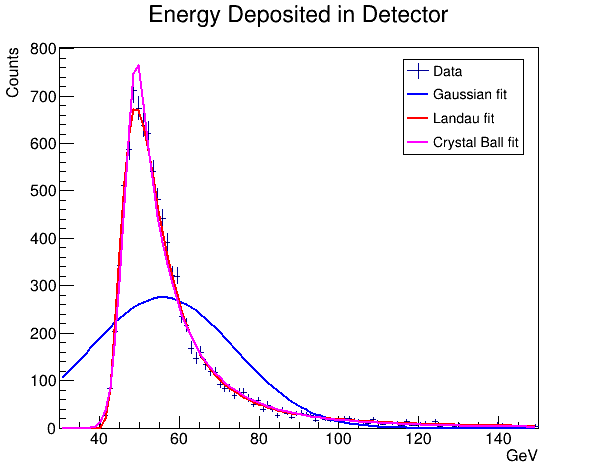
\includegraphics[width=\textwidth]{fit.png}
    \caption{Fits to the smeared energy deposition data. The data (error bars) is overlaid with a Gaussian fit (blue), Landau fit (red), and Crystal Ball fit (magenta).}
    \label{fig:fit}
    \end{figure}
    \vspace{1.5cm}

The parameters for each of the fits were as follows:

\begin{itemize}
    \item Gaussian fit: Constant = 275.361, Mean = 55.7785, Sigma = 18.2588.
    \item Landau fit: Constant = 3739.53, MPV = 49.8687, Sigma = 3.21775.
    \item Crystal Ball fit: Constant = 770.09, Mean = 49.3842, Sigma = 3.24137, Alpha = -0.408838, N = 3.80958.
\end{itemize}

\section*{Conclusion}

Based on the chi-square values, we find that the Landau function provides the best fit to the data. This result indicates that our model of energy deposition as a Landau distribution is indeed a good model for the physical process. 

However, the Crystal Ball function also provides a good fit, suggesting that there might be some large energy deposition events influencing the detector response. This insight could be useful in improving the design or operation of the detector. With tuning of the crystal ball function, for instance, tweaking the initial parameter estimates for normalization, this fit might actually outperform the Landau fit. 

In conclusion, this simulation provides a useful procedure for studying the behavior of particle detectors and the uncertainties associated with their measurements. It demonstrates the importance of choosing an appropriate model for the physical process (Landau far outperforms Gaussian) and that sometimes two models might have very close fits to the data, in this case it was a close competition between Landau and crystal ball function fits.
\end{document}